\\
\\
\section{Feature model}

As a second approach, the  Fiure \ref{fig:featureModel} shows the core features of the application, showing which of them are mandatory and which of them are optional.


\clearpage

\afterpage{%
    \clearpage% Flush earlier floats (otherwise order might not be correct)
    \thispagestyle{empty}% empty page style (?)
    \begin{landscape}

\begin{figure}[h!]
    \centering
    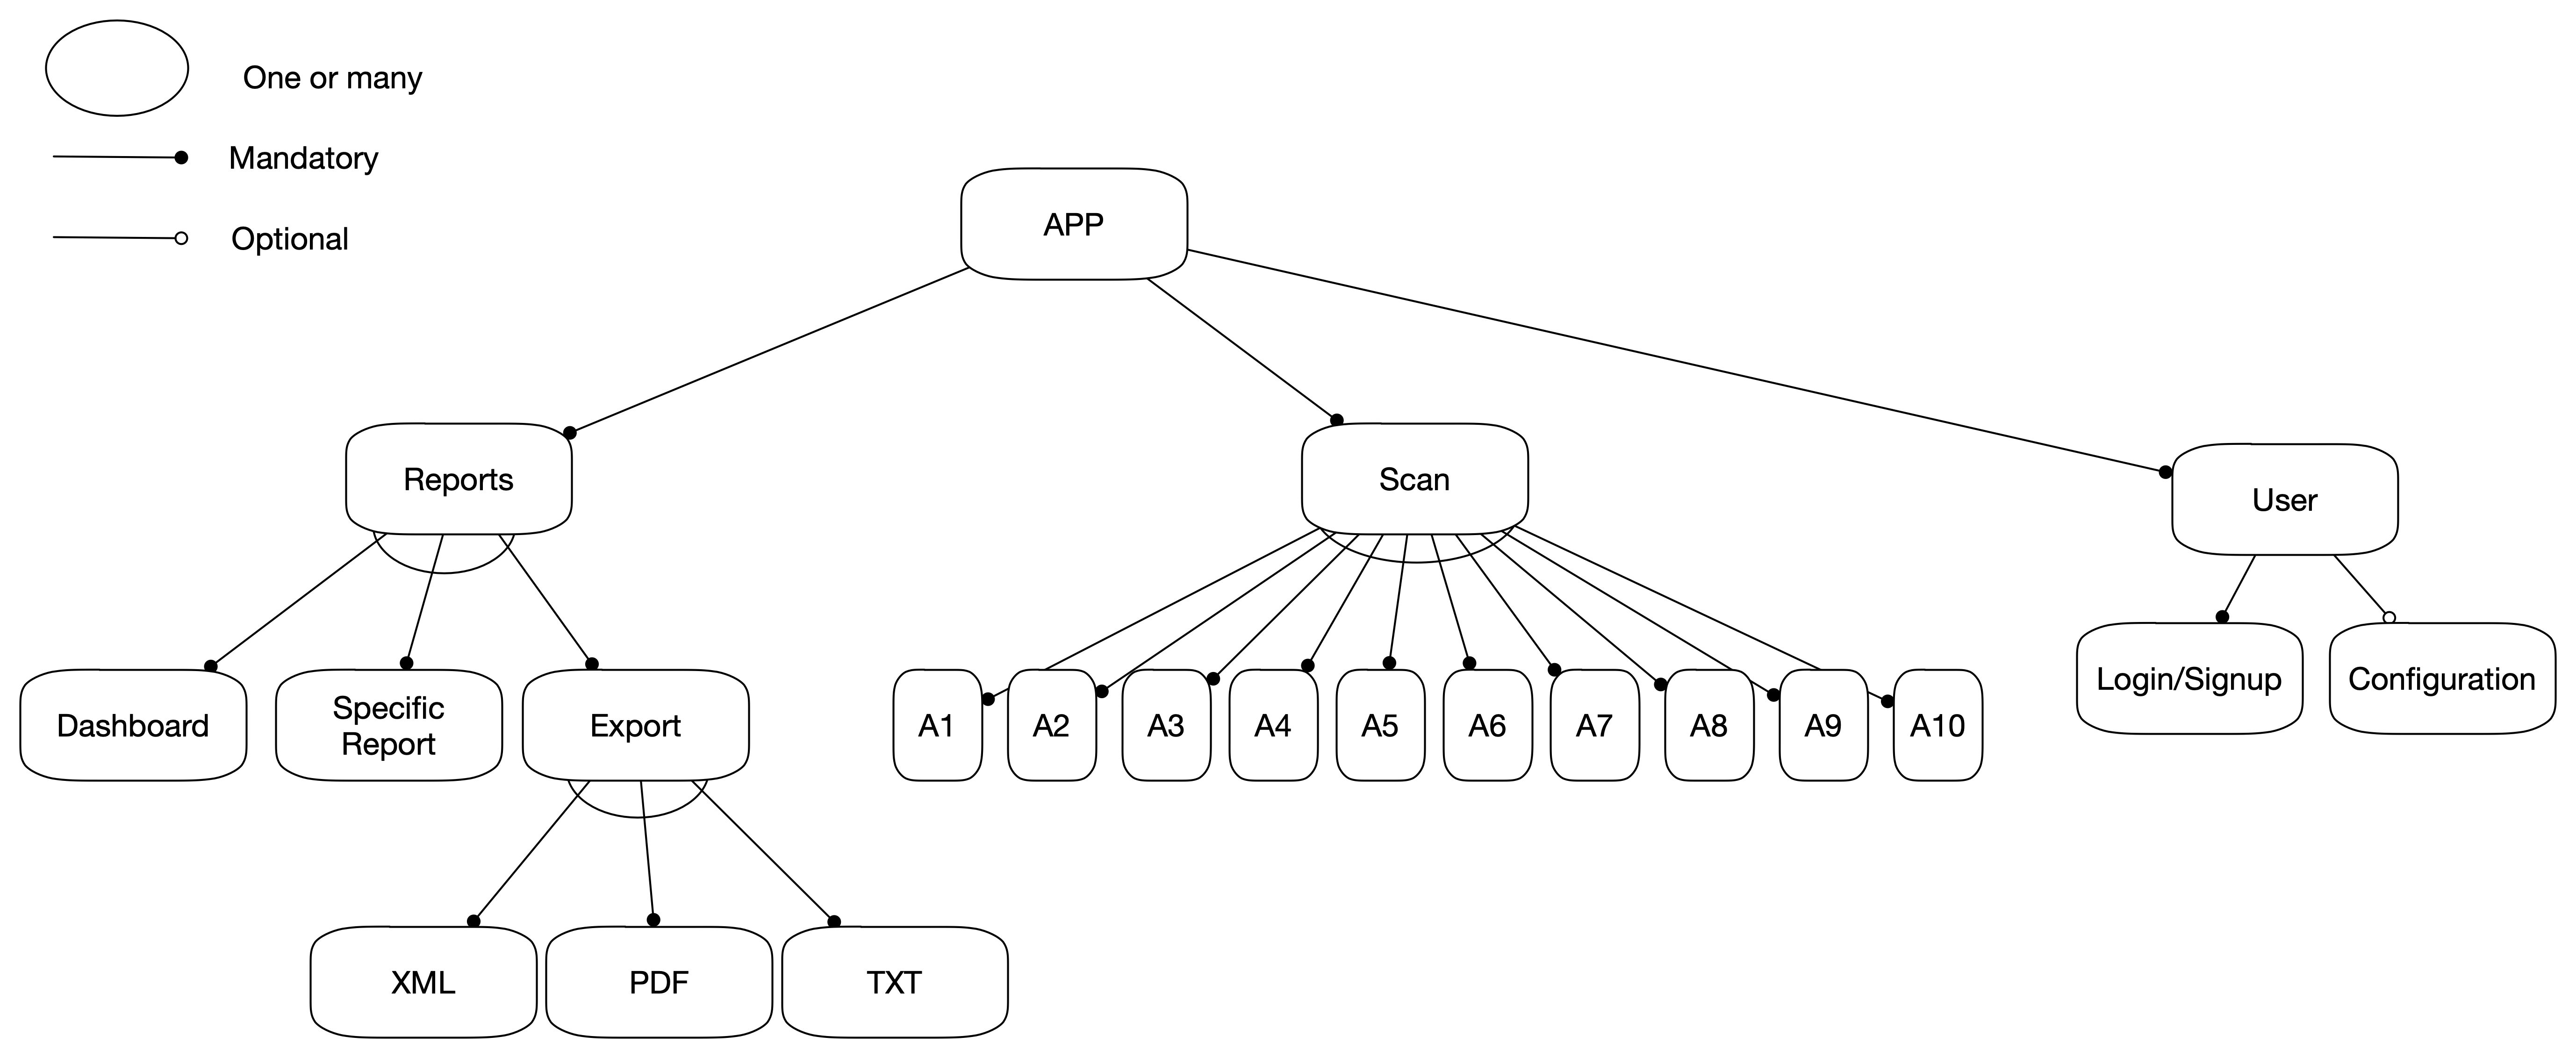
\includegraphics[width=25cm]{img/featureModel.jpg}
    \caption{Feature model}
    \label{fig:featureModel}
\end{figure}


    
    \end{landscape}

    \clearpage% Flush page
}

\clearpage